\chapter{Mathematik}
\section{05.11.2008}
\subsection{05.11.2008-IMG-mathe-4}
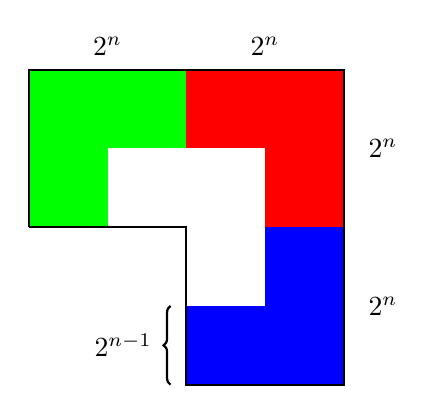
\begin{tikzpicture}[thick]
	\fill[fill=green] (0,0) rectangle (1,2);
	\fill[fill=green] (1,2) rectangle (2,1);

	\fill[fill=red] (2,2) rectangle (4,1);
	\fill[fill=red] (3,1) rectangle (4,0);

	\fill[fill=blue] (3,0) rectangle (4,-2);
	\fill[fill=blue] (3,-2) rectangle (2,-1);

	\draw (0,0) -- (2,0) -- (2,-2) -- (4,-2) -- (4,2) -- (0,2) -- (0,0);

	\node at (1,2.3) {$2^n$};
	\node at (3,2.3) {$2^n$};
	\node at (4.5,1) {$2^n$};
	\node at (4.5,-1) {$2^n$};
	\draw decorate [decoration=brace] {(1.8,-2) -- (1.8,-1)};
	\node at (1.2,-1.5) {$2^{n-1}$};
\end{tikzpicture}
\begin{lstlisting}[frame=single]
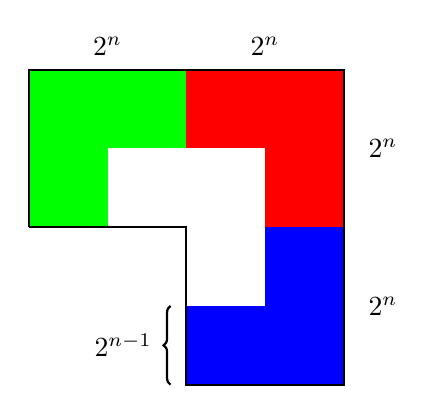
\begin{tikzpicture}[thick]
	\fill[fill=green] (0,0) rectangle (1,2);
	\fill[fill=green] (1,2) rectangle (2,1);

	\fill[fill=red] (2,2) rectangle (4,1);
	\fill[fill=red] (3,1) rectangle (4,0);

	\fill[fill=blue] (3,0) rectangle (4,-2);
	\fill[fill=blue] (3,-2) rectangle (2,-1);

	\draw (0,0) -- (2,0) -- (2,-2) -- (4,-2) -- (4,2) -- (0,2) -- (0,0);

	\node at (1,2.3) {$2^n$};
	\node at (3,2.3) {$2^n$};
	\node at (4.5,1) {$2^n$};
	\node at (4.5,-1) {$2^n$};
	\draw decorate [decoration=brace] {(1.8,-2) -- (1.8,-1)};
	\node at (1.2,-1.5) {$2^{n-1}$};
\end{tikzpicture}
\end{lstlisting}

\subsection{05.11.2008-IMG-mathe-5}
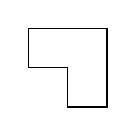
\begin{tikzpicture}
	\draw (0,0) -- (0,0.5) -- (1,0.5) -- (1,-0.5) -- (0.5,-0.5) -- (0.5,0) -- (0,0);
\end{tikzpicture}
\begin{lstlisting}[frame=single]
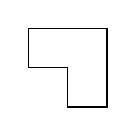
\begin{tikzpicture}
	\draw (0,0) -- (0,0.5) -- (1,0.5) -- (1,-0.5) -- (0.5,-0.5) -- (0.5,0) -- (0,0);
\end{tikzpicture}
\end{lstlisting}

\subsection{05.11.2008-IMG-mathe-6}
\begin{tikzpicture}
	\draw (0,0) rectangle (0.5,0.5);

	\node at (0.25,0.8) {$1$};
	\node at (0.8,0.25) {$1$};
\end{tikzpicture}
\begin{lstlisting}[frame=single]
\begin{tikzpicture}
	\draw (0,0) rectangle (0.5,0.5);

	\node at (0.25,0.8) {$1$};
	\node at (0.8,0.25) {$1$};
\end{tikzpicture}
\end{lstlisting}

\subsection{05.11.2008-IMG-mathe-7}
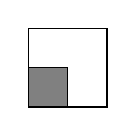
\begin{tikzpicture}
	\draw (0,0) rectangle (1,1);
	\draw[fill=gray] (0,0) rectangle (0.5,0.5);
\end{tikzpicture}
\begin{lstlisting}[frame=single]
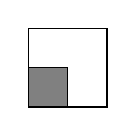
\begin{tikzpicture}
	\draw (0,0) rectangle (1,1);
	\draw[fill=gray] (0,0) rectangle (0.5,0.5);
\end{tikzpicture}
\end{lstlisting}

\subsection{05.11.2008-IMG-mathe-8}
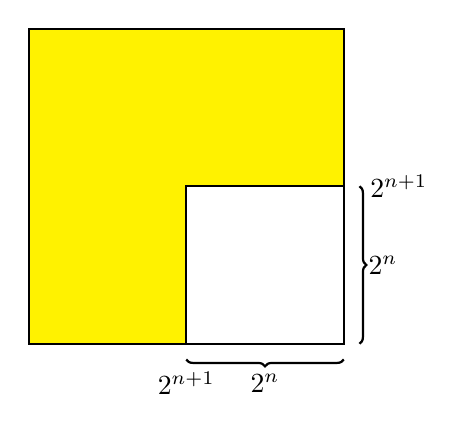
\begin{tikzpicture}[thick]
	\draw[fill=yellow] (0,0) rectangle (4,4);
	\draw[fill=white] (2,2) rectangle (4,0);

	\draw decorate [decoration=brace]  {(4,-0.2) -- (2,-0.2)};
	\draw decorate [decoration=brace] {(4.2,2) -- (4.2,0)};

	\node at (2,-0.5) {$2^{n+1}$};
	\node at (4.7,2) {$2^{n+1}$};
	\node at (3,-0.5) {$2^n$};
	\node at (4.5,1) {$2^n$};
\end{tikzpicture}
\begin{lstlisting}[frame=single]
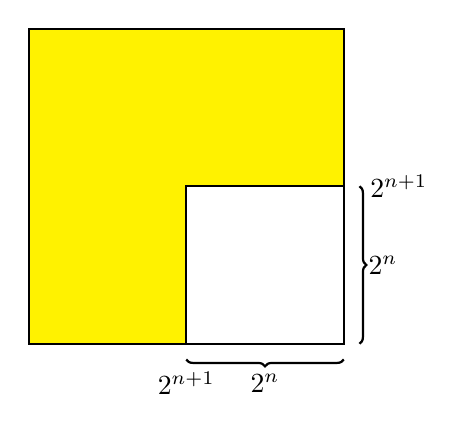
\begin{tikzpicture}[thick]
	\draw[fill=yellow] (0,0) rectangle (4,4);
	\draw[fill=white] (2,2) rectangle (4,0);

	\draw decorate [decoration=brace]  {(4,-0.2) -- (2,-0.2)};
	\draw decorate [decoration=brace] {(4.2,2) -- (4.2,0)};

	\node at (2,-0.5) {$2^{n+1}$};
	\node at (4.7,2) {$2^{n+1}$};
	\node at (3,-0.5) {$2^n$};
	\node at (4.5,1) {$2^n$};
\end{tikzpicture}
\end{lstlisting}

\subsection{05.11.2008-IMG-mathe-9}

\begin{tikzpicture}
	\fill[fill=yellow] (0,0) rectangle (0.5,1);
	\fill[fill=yellow] (0.5,1) rectangle (1,0.5);
	\draw (0,0) -- (0,1) -- (1,1) -- (1,0.5) -- (0.5,0.5) -- (0.5,0) -- (0,0);
\end{tikzpicture}
\begin{lstlisting}[frame=single]

\begin{tikzpicture}
	\fill[fill=yellow] (0,0) rectangle (0.5,1);
	\fill[fill=yellow] (0.5,1) rectangle (1,0.5);
	\draw (0,0) -- (0,1) -- (1,1) -- (1,0.5) -- (0.5,0.5) -- (0.5,0) -- (0,0);
\end{tikzpicture}
\end{lstlisting}

\subsection{05.11.2008-IMG-mathe-10}
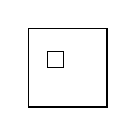
\begin{tikzpicture}
	\draw (0,0) rectangle (1,1);
	\draw (0.25,0.5) rectangle (0.45,0.7);
\end{tikzpicture}
\begin{lstlisting}[frame=single]
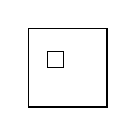
\begin{tikzpicture}
	\draw (0,0) rectangle (1,1);
	\draw (0.25,0.5) rectangle (0.45,0.7);
\end{tikzpicture}
\end{lstlisting}

\subsection{IMG-05.11.2008-mathe-3}
\begin{tikzpicture}
	\draw (0,0) -- (2,0) -- (2,-2) -- (4,-2) -- (4,2) -- (0,2) -- (0,0);

	\draw[dashed] (2,0) -- (2,2);
	\draw[dashed] (2,0) -- (4,0);

	\node at (1,2.3) {$2^{n-1}$};
	\node at (3,2.3) {$2^{n-1}$};
	\node at (4.5,1) {$2^{n-1}$};
	\node at (4.5,-1) {$2^{n-1}$};
\end{tikzpicture}
\begin{lstlisting}[frame=single]
\begin{tikzpicture}
	\draw (0,0) -- (2,0) -- (2,-2) -- (4,-2) -- (4,2) -- (0,2) -- (0,0);

	\draw[dashed] (2,0) -- (2,2);
	\draw[dashed] (2,0) -- (4,0);

	\node at (1,2.3) {$2^{n-1}$};
	\node at (3,2.3) {$2^{n-1}$};
	\node at (4.5,1) {$2^{n-1}$};
	\node at (4.5,-1) {$2^{n-1}$};
\end{tikzpicture}
\end{lstlisting}

\section{11.12.2008}
\subsection{11.12.2008-IMG-mathe-1}
\definecolor{lightergray}{HTML}{DDDDDD}
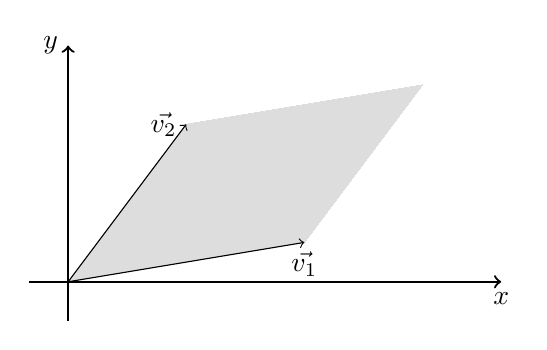
\begin{tikzpicture}
	\draw[fill=lightergray, line width=0pt, draw=lightergray] (0,0) -- (1.5,2) -- (4.5,2.5) -- (3,0.5) -- (0,0);

	\draw[->] (0,0) -- (1.5,2) node[left] {$\vec{v_2}$};
	\draw[->] (0,0) -- (3,0.5) node[below] {$\vec{v_1}$};

	\draw[->, thick] (-0.5,0) -- (5.5,0) node[below] {$x$};
	\draw[->, thick] (0,-0.5) -- (0,3) node[left] {$y$};
\end{tikzpicture}
\begin{lstlisting}[frame=single]
\definecolor{lightergray}{HTML}{DDDDDD}
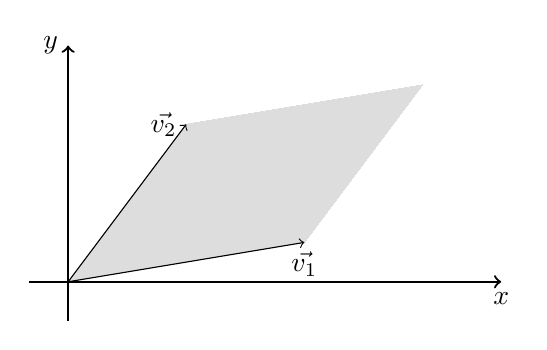
\begin{tikzpicture}
	\draw[fill=lightergray, line width=0pt, draw=lightergray] (0,0) -- (1.5,2) -- (4.5,2.5) -- (3,0.5) -- (0,0);

	\draw[->] (0,0) -- (1.5,2) node[left] {$\vec{v_2}$};
	\draw[->] (0,0) -- (3,0.5) node[below] {$\vec{v_1}$};

	\draw[->, thick] (-0.5,0) -- (5.5,0) node[below] {$x$};
	\draw[->, thick] (0,-0.5) -- (0,3) node[left] {$y$};
\end{tikzpicture}
\end{lstlisting}

\subsection{11.12.2008-IMG-mathe-2}
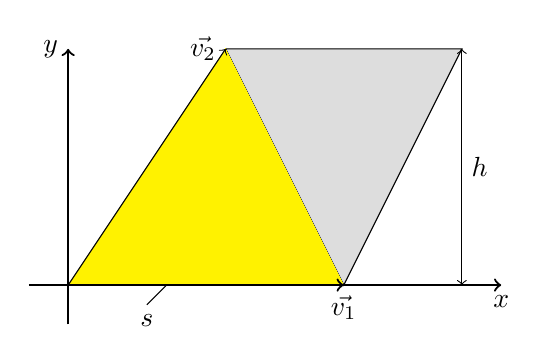
\begin{tikzpicture}
	\draw[fill=lightergray] (2,3) -- (3.5,0) -- (5,3) -- (2,3); 

	\draw[fill=yellow, line width=0pt, draw=yellow] (0,0) -- (2,3) -- (3.5,0) -- (0,0);

	\draw[->] (0,0) -- (2,3) node[left] {$\vec{v_2}$};
	\draw[->, thick] (0,0) -- (3.5,0) node[below] {$\vec{v_1}$};
	\draw (1.25,0) -- (1,-0.25) node[below] {$s$};
	\draw[<->] (5,3) -- (5,0);
	\node[right] at (5,1.5) {$h$};

	\draw[->, thick] (-0.5,0) -- (5.5,0) node[below] {$x$};
	\draw[->, thick] (0,-0.5) -- (0,3) node[left] {$y$};
\end{tikzpicture}
\begin{lstlisting}[frame=single]
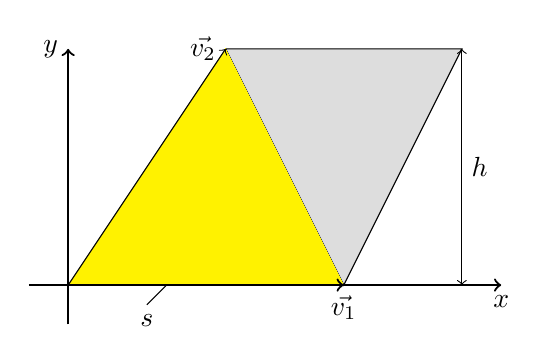
\begin{tikzpicture}
	\draw[fill=lightergray] (2,3) -- (3.5,0) -- (5,3) -- (2,3); 

	\draw[fill=yellow, line width=0pt, draw=yellow] (0,0) -- (2,3) -- (3.5,0) -- (0,0);

	\draw[->] (0,0) -- (2,3) node[left] {$\vec{v_2}$};
	\draw[->, thick] (0,0) -- (3.5,0) node[below] {$\vec{v_1}$};
	\draw (1.25,0) -- (1,-0.25) node[below] {$s$};
	\draw[<->] (5,3) -- (5,0);
	\node[right] at (5,1.5) {$h$};

	\draw[->, thick] (-0.5,0) -- (5.5,0) node[below] {$x$};
	\draw[->, thick] (0,-0.5) -- (0,3) node[left] {$y$};
\end{tikzpicture}
\end{lstlisting}

\subsection{11.12.2008-IMG-mathe-3}
\begin{tikzpicture}
	\draw[->, thick] (0,0) -- (6,0) node[right] {$y$};
	\draw[->, thick] (0,0) -- (0,7) node[left] {$z$};
	\draw[->, thick] (0,0) -- (-2,-2.5) node[below] {$x$};

	\draw[draw=gray, nearly opaque, thick] (-1,-2) -- (-1,4) -- (2,4) -- (2,-2) -- (-1,-2);
	\draw[draw=gray, nearly opaque, thick] (-1,4) -- (1,6) -- (4,6) -- (2,4);
	\draw[draw=gray, nearly opaque, thick] (2,-2) -- (4,0) -- (4,6) node [above] {\LARGE{$V$}};
\end{tikzpicture}
\begin{lstlisting}[frame=single]
\begin{tikzpicture}
	\draw[->, thick] (0,0) -- (6,0) node[right] {$y$};
	\draw[->, thick] (0,0) -- (0,7) node[left] {$z$};
	\draw[->, thick] (0,0) -- (-2,-2.5) node[below] {$x$};

	\draw[draw=gray, nearly opaque, thick] (-1,-2) -- (-1,4) -- (2,4) -- (2,-2) -- (-1,-2);
	\draw[draw=gray, nearly opaque, thick] (-1,4) -- (1,6) -- (4,6) -- (2,4);
	\draw[draw=gray, nearly opaque, thick] (2,-2) -- (4,0) -- (4,6) node [above] {\LARGE{$V$}};
\end{tikzpicture}
\end{lstlisting}

\section{08.01.2009}
\subsection{08.01.2009-IMG-math-1}
%Picture
\begin{tikzpicture}
	\node at (0,0) (Vl) {$V$};
	\node at (3,0) (Vr) {$V$};
	\node at (0,3) (Kl) {$K^n$};
	\node at (3,3) (Kr) {$K^n$};

	\draw[->] (Vl.north) -- (Kl.south);
	\draw[->] (Vl.east) -- (Vr.west) node[above, midway] {$f$};

	\draw[->] (Kl.east) -- (Kr.west) node[below, midway] {$f$};

	\draw[->] (Kr.south) -- (Vr.north);
\end{tikzpicture}
%Code
\begin{lstlisting}[frame=single]
\begin{tikzpicture}
	\node at (0,0) (Vl) {$V$};
	\node at (3,0) (Vr) {$V$};
	\node at (0,3) (Kl) {$K^n$};
	\node at (3,3) (Kr) {$K^n$};

	\draw[->] (Vl.north) -- (Kl.south);
	\draw[->] (Vl.east) -- (Vr.west) node[above, midway] {$f$};

	\draw[->] (Kl.east) -- (Kr.west) node[below, midway] {$f$};

	\draw[->] (Kr.south) -- (Vr.north);
\end{tikzpicture}
\end{lstlisting}

\section{14.01.2009}
\subsection{14.01.2009-IMG-mathe-1}
%Picture
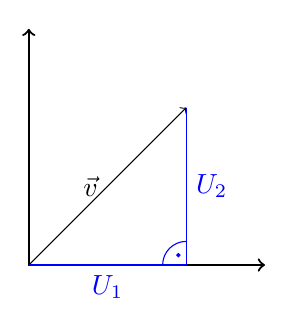
\begin{tikzpicture}
	\draw[thick, <->] (3,0) -- (0,0) -- (0,3);

	\draw[->] (0,0) -- (2,2) node[left, midway] {$\vec{v}$};
	\draw[draw=blue, thick] (0,0) -- (2,0) node[below, midway, text=blue] {$U_1$};
	\draw[draw=blue] (2,0) -- (2,2) node[right, midway, text=blue] {$U_2$};
	\draw[draw=blue] (1.7,0) arc (180:90:0.3);
	\draw[draw=blue, fill=blue] (1.9,0.125) circle (0.02);
\end{tikzpicture}
%Code
\begin{lstlisting}[frame=single]
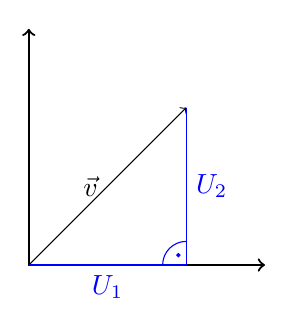
\begin{tikzpicture}
	\draw[thick, <->] (3,0) -- (0,0) -- (0,3);

	\draw[->] (0,0) -- (2,2) node[left, midway] {$\vec{v}$};
	\draw[draw=blue, thick] (0,0) -- (2,0) node[below, midway, text=blue] {$U_1$};
	\draw[draw=blue] (2,0) -- (2,2) node[right, midway, text=blue] {$U_2$};
	\draw[draw=blue] (1.7,0) arc (180:90:0.3);
	\draw[draw=blue, fill=blue] (1.9,0.125) circle (0.02);
\end{tikzpicture}
\end{lstlisting}

\subsection{14.01.2009-IMG-mathe-2}
%Picture
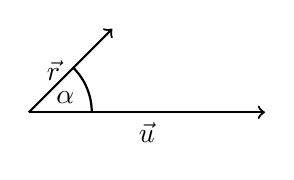
\begin{tikzpicture}
	\draw[->, thick] (0,0) -- (3,0) node[below, midway] {$\vec{u}$};
	\draw[->, thick] (0,0) -- (45:1.5) node[left, midway] {$\vec{r}$};
	\draw[thick] (0.8,0) arc (0:45:0.8);
	\path (0,0) ++(22.5:0.5) node{$\alpha$};
\end{tikzpicture}
%Code
\begin{lstlisting}[frame=single]
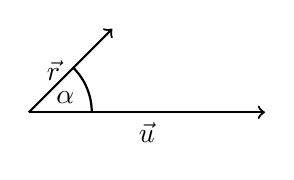
\begin{tikzpicture}
	\draw[->, thick] (0,0) -- (3,0) node[below, midway] {$\vec{u}$};
	\draw[->, thick] (0,0) -- (45:1.5) node[left, midway] {$\vec{r}$};
	\draw[thick] (0.8,0) arc (0:45:0.8);
	\path (0,0) ++(22.5:0.5) node{$\alpha$};
\end{tikzpicture}
\end{lstlisting}

\subsection{14.01.2009-IMG-mathe-3}
%Picture
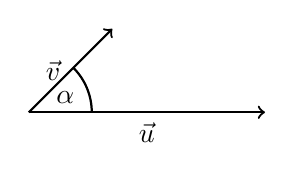
\begin{tikzpicture}
	\draw[->, thick] (0,0) -- (3,0) node[below, midway] {$\vec{u}$};
	\draw[->, thick] (0,0) -- (45:1.5) node[left, midway] {$\vec{v}$};
	\draw[thick] (0.8,0) arc (0:45:0.8);
	\path (0,0) ++(22.5:0.5) node{$\alpha$};
\end{tikzpicture}
%Code
\begin{lstlisting}[frame=single]
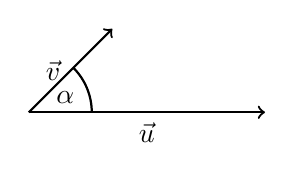
\begin{tikzpicture}
	\draw[->, thick] (0,0) -- (3,0) node[below, midway] {$\vec{u}$};
	\draw[->, thick] (0,0) -- (45:1.5) node[left, midway] {$\vec{v}$};
	\draw[thick] (0.8,0) arc (0:45:0.8);
	\path (0,0) ++(22.5:0.5) node{$\alpha$};
\end{tikzpicture}
\end{lstlisting}

\subsection{14.01.2009-IMG-mathe-4}
%Picture
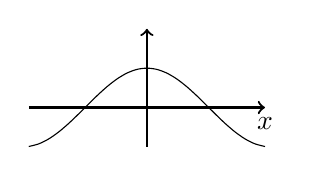
\begin{tikzpicture}
	\draw[->, thick] (-1.5,0) -- (1.5,0) node[below] {$x$};
	\draw[->, thick] (0,-0.5) -- (0,1);
	\draw[smooth] plot[domain=-3:3, scale=0.5] (\x,{cos(\x r)});
\end{tikzpicture}
%Code
\begin{lstlisting}[frame=single]
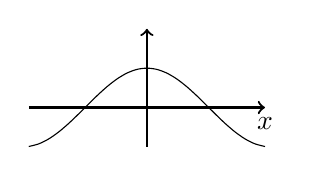
\begin{tikzpicture}
	\draw[->, thick] (-1.5,0) -- (1.5,0) node[below] {$x$};
	\draw[->, thick] (0,-0.5) -- (0,1);
	\draw[smooth] plot[domain=-3:3, scale=0.5] (\x,{cos(\x r)});
\end{tikzpicture}
\end{lstlisting}

\section{15.01.2009}
\subsection{15.01.2009-IMG-mathe-1}
%Picture
\begin{tikzpicture}
	\draw[<->, thick] (0,3) -- (0,0) node[left, midway] {$\vec{v}$} -- (5,0) node[below, midway] {$\vec{u}$};
	\draw[thick] (0,0.5) arc (90:0:0.5);
	\path (0,0) ++(45:0.25) node{$\alpha$};
\end{tikzpicture}
%Code
\begin{lstlisting}[frame=single]
\begin{tikzpicture}
	\draw[<->, thick] (0,3) -- (0,0) node[left, midway] {$\vec{v}$} -- (5,0) node[below, midway] {$\vec{u}$};
	\draw[thick] (0,0.5) arc (90:0:0.5);
	\path (0,0) ++(45:0.25) node{$\alpha$};
\end{tikzpicture}
\end{lstlisting}

\subsection{15.01.2009-IMG-mathe-2}
%Picture
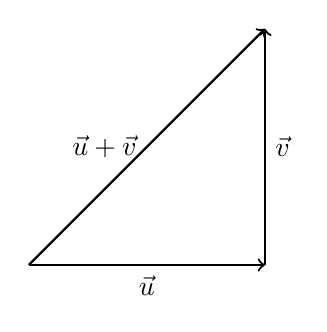
\begin{tikzpicture}
	\draw[->, thick] (0,0) -- (3,3) node[left, midway] {$\vec{u} + \vec{v}$};
	\draw[->, thick] (0,0) -- (3,0) node[below, midway] {$\vec{u}$};
	\draw[->, thick] (3,0) -- (3,3) node[right, midway] {$\vec{v}$};
\end{tikzpicture}
%Code
\begin{lstlisting}[frame=single]
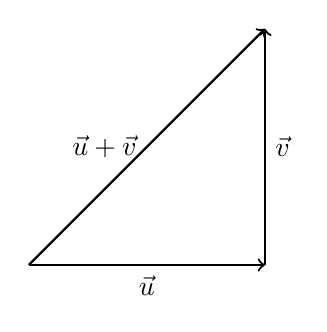
\begin{tikzpicture}
	\draw[->, thick] (0,0) -- (3,3) node[left, midway] {$\vec{u} + \vec{v}$};
	\draw[->, thick] (0,0) -- (3,0) node[below, midway] {$\vec{u}$};
	\draw[->, thick] (3,0) -- (3,3) node[right, midway] {$\vec{v}$};
\end{tikzpicture}
\end{lstlisting}

\subsection{15.01.2009-IMG-mathe-3}
%Picture
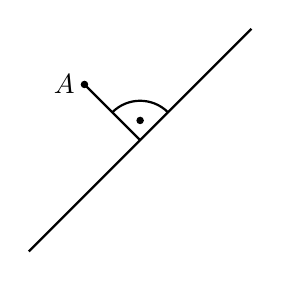
\begin{tikzpicture}
	\draw[thick] (0,0) -- (45:4);
	\draw[thick] (45:2) -- +(135:1);
	\draw[fill=black] (45:2) ++ (135:1) circle (0.04) node[left] {$A$};
	\draw[thick] (45:2) ++ (135:0.5) arc (135:45:0.5);
	\draw[fill=black] (45:2) ++ (90:0.25) circle (0.04);
\end{tikzpicture}
%Code
\begin{lstlisting}[frame=single]
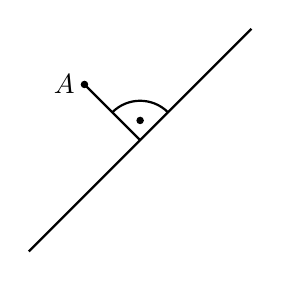
\begin{tikzpicture}
	\draw[thick] (0,0) -- (45:4);
	\draw[thick] (45:2) -- +(135:1);
	\draw[fill=black] (45:2) ++ (135:1) circle (0.04) node[left] {$A$};
	\draw[thick] (45:2) ++ (135:0.5) arc (135:45:0.5);
	\draw[fill=black] (45:2) ++ (90:0.25) circle (0.04);
\end{tikzpicture}
\end{lstlisting}
